\section{Browser-Technologien}
Vordefinierte Objekte

\begin{itemize}
  \item Die allgemeinen Objekte sind in JavaScript vordefiniert
  \item Tatsächlich handelt es sich um Funktionen/Konstruktoren
  \item Die Browser-Objekte existieren auf der Browser-Plattform
  \item Sie beziehen sich auf das Browser-Fenster, das angezeigte Dokument, oder den Browser selbst\\
document
  \item Repräsentiert die angezeigte Webseit
  \item Einstieg ins DOM (Document Object Model)
  \item Diverse Attribute und Methoden, zum Beispiel:
\end{itemize}

\begin{verbatim}
1 document.cookie /* Zugriff auf Cookies */
2 document.lastModified /* Zeit der letzten Änderung */
3 document.links /* die Verweise der Seite */
4 |document.images /* die Bilder der Seite */
\end{verbatim}

window

\begin{itemize}
  \item Repräsentiert das Browserfenster
  \item Zahlreiche Attribute und Methoden, u.a.:
  \item Alle globalen Variablen und Methoden sind hier angehängt
  \item Neue globale Variablen landen ebenfalls hier
\end{itemize}

\begin{verbatim}
1 window.document /* Zugriff auf Dokument */
2 window.history /* History-Objekt */
3 window.innerHeight /* Höhe des Viewports */
4 window.pageYOffset /* vertikal gescrollte Pixel */
5 window.alert === alert /* -> true */
6 window.setTimeout === setTimeout /* -> true */
7 window.parseInt === parseInt /* true */
\end{verbatim}

\section*{navigator}
Konsolen-eingabe auf dem folgenden Bild:

\begin{verbatim}
> navigator.userAgent
"Mozilla/5.0 (Macintosh; Intel Mac OS X 10.15; rv:91.0) Gecko/20100101 Firefox/91.0"
> navigator.language
"de"
> navigator.platform
"MacIntel"
> navigator.onLine
true
location
> location.href
"https://gburkert.github.io/selectors/"
> location.protocol
"https:"
> document.location.protocol
"https:"
\end{verbatim}

\subsection{JavaScript und DOM}

\begin{itemize}
    \item Element erzeugen: document.createElement
    \item Attribute erzeugen: document.createAttribute
    \item Und hinzufügen: .setAttribute
    \item Element in Baum einfügen: .appendChild
  \end{itemize}
  
  Element auffinden
  
  \begin{verbatim}
  1 let aboutus = document.getElementById("aboutus")
  2 let aboutlinks = aboutus.getElementsByTagName("a")
  3 let aboutimportant = aboutus.getElementsByClassName("important")
  4 let navlinks = document.querySelectorAll("nav a")
  \end{verbatim}
  
  \section*{Textknoten erzeugen}
  \begin{verbatim}
  <p>The <img src="img/cat.png" alt="Cat"> in the
  <img src="img/hat.png" alt="Hat">.</p>
  <p><button onclick="replaceImages()">Replace</button></p>
  <script>
      function replaceImages () {
          let images = document.body.getElementsByTagName("img")
          for (let i = images.length - 1; i >= 0; i--) {
                  let image = images[i]
                  if (image.alt) {
                  let text = document.createTextNode(image.alt)
                  image.parentNode.replaceChild(text, image)
                  }
              }
      }
  </script>
  \end{verbatim}
  
  Elementknoten erzeugen
  
  \begin{verbatim}
  <blockquote id="quote">
      No book can ever be finished. While working on it we learn ...
  </blockquote>
  <script>
  /* definition of elt ... */
  document.getElementById("quote").appendChild(
      elt("footer", "-",
      elt("strong", "Karl Popper"),
      ", preface to the second edition of ",
      elt("em", "The Open Society and Its Enemies"),
      ", 1950"))
  </script>
  \end{verbatim}
  
  Attribut setzen\\
  1
  
  6
  
  8
  
  \begin{verbatim}
  3 let att = document.createAttribute("class")
  4 att.value ="democlass"
  5 h1.setAttributeNode(att)
  7 /* oder kürzer: */
  let h1 = document.querySelector("h1")
  ,h1.setAttribute("class","democlass")
  \end{verbatim}
  
  Style anpassen\\
  1 Nice text\\
  2 
  
  \section*{Event handling}
  Event abonnieren/entfernen\\
  Mit der Methode addEventListener() wird ein Event abonniert. Mit removeEventListener kann das Event entfernt werden.
  
  \begin{verbatim}
  <button>Act-once button</button>
  <script>
      let button = document.querySelector("button")
      function once () {
          console.log("Done.")
          button.removeEventListener("click", once)
      }
      button.addEventListener("click", once)
  </script>
  \end{verbatim}
  
  Wenn ein Parameter zur Methode hinzugefügt wird, wird dieses als das Event-Objekt gesetzt.
  
  \begin{verbatim}
  <script>
      let button = document.querySelector("button")
      button.addEventListener("click", (e) => {
          console.log("x="+e.x+", y="+e.y)
      })
  </script\
  \end{verbatim}
  
  Das Event wird bei allen abonnierten Handlern ausgeführt bis ein Handler stopPropagation() ausführt.
  
  \begin{verbatim}
  <script>
      let button = document.querySelector("button")
      button.addEventListener("click", (e) => {
                  console.log("x="+e.x+", y="+e.y)
                  e.stopPropagation()
      })
  </script>
  \end{verbatim}
  
  Viele Ereignisse haben ein Default verhalten. Eigene Handler werden vor Default-Verhalten ausgeführt. Um das Default-Verhalten zu verhindern, muss die Methode preventDefault() ausgeführt werden.
  
  \begin{verbatim}
  <a href="https://developer.mozilla.org/">MDN</a>
  <script>
      let link = document.querySelector("a")
      link.addEventListener("click", event => {
              console.log("Nope.")
                  event.preventDefault()
          })
  ,/script>
  \end{verbatim}
  
  \section*{Tastatur-Events}
  \begin{itemize}
    \item keydown
    \item keyup
    \item Achtung: bei keydown kann das event mehrfach ausgelöst werden
  \end{itemize}
  
  \begin{verbatim}
  <p>Press Control-Space to continue.</p>
  <script>
      window.addEventListener("keydown", event => {
              if (event.key ==" " && event.ctrlKey) {
                  console.log("Continuing!")
              }
      })
  </script>
  \end{verbatim}
  
  Mauszeiger-Events
  
  \begin{itemize}
    \item Mausklicks:
    \item mousedown
    \item mouseup
    \item click
    \item dblclick
    \item Mausbewegung
    \item mousemove
    \item Touch-display
    \item touchstart
    \item touchmove
    \item touched
  \end{itemize}
  
  \section*{Scroll-Events}
  Das Scrollevent hat die Attribute des Event-Objekts: pageYOffset, pageXOffset.
  
  \begin{verbatim}
  window.addEventListener("scroll", () => {
      let max = document.body.scrollHeight - innerHeight
      bar.style.width = `${(pageYOffset / max) * 100}%`
  ,})
  \end{verbatim}
  
  Fokus- und Ladeereignisse
  
  \begin{itemize}
    \item Fokus erhalten / verlieren
    \item focus
    \item blur
    \item Seite wurde geladen (ausgelöst auf window und document.body)
    \item load
    \item beforeunload
  \end{itemize}
  
  Jquery\\
  JQuery ist eine freie JavaScript-Bibliothek, die Funktionen zur DOM-Navigation und -Manipulation zur Verfügung stellt.
  
  \begin{verbatim}
  $("button.continue").html("Next Step...")
  var hiddenBox = $("#banner-message")
  $("#button-container button").on("click", function(event) {
          hiddenBox.show()
      .})
  \end{verbatim}
  
  \begin{center}
  \begin{tabular}{|c|c|c|}
  \hline
  Aufruf & Bedeutung & Beispiel \\
  \hline
  \$(Funktion) & DOM ready & \$(function0 \{ .... \}); \\
  \hline
  \multirow[t]{4}{*}{\$("CSS Selektor" ) .aktion(arg1, ....) .aktion(...)} & Wrapped Set & \$(".toggleButton").attr("title") \\
  \hline
   & - Knoten, die Sel. erfüllen & \$(".toggleButton").attr("title", "click here") \\
  \hline
   & - eingepackt in jQuery Obj. & \$(".toggleButton").attr((fitiel : "click here", ...)) \\
  \hline
   &  & \texttt{\$(".toggleButton").attr("title", function0\{...\}) .css(...) .text(..) on("click", function(event) \{ ...\})} \\
  \hline
  \multirow[t]{2}{*}{\$("HTML-Code" )} & \begin{tabular}{l}
  Wrapped Set \\
  - neuer Knoten \\
  \end{tabular} & \$("...").addClass(...) .appendTo("Selektor") \\
  \hline
   & \begin{tabular}{l}
  - eingepackt in jQuery Obj. \\
  - noch nicht im DOM \\
  \end{tabular} & \$("<li>>-.../li>").length \$("<li>...<li>")[0] \\
  \hline
  \multirow[t]{2}{*}{\$(DOM-Knoten)} & Wrapped Set & \$(document.body) \\
  \hline
   & \begin{tabular}{l}
  - dieser Knoten \\
  - eingepackt in jQuery Obj. \\
  \end{tabular} & \$(this) \\
  \hline
  \end{tabular}
  \end{center}
  
  \section*{Web-Grafiken}
  \begin{itemize}
    \item Einfache Grafiken mit HTML und CSS möglich
    \item Zum Beispiel: Balkendiagramme
    \item Alternative für Vektorgrafiken: SVG
    \item Alternative für Pixelgrafiken: Canvas
  \end{itemize}
  
  SVG
  
  \begin{itemize}
    \item Basiert wie HTML auf XML
    \item Elemente repräsentieren grafische Formen
    \item Ins DOM integriert und durch Scripts anpassbar
  \end{itemize}
  
  Beispiel:
  
  \begin{verbatim}
  p>Normal HTML here.</p>
  <svg xmlns="http://www.w3.org/2000/svg">
      <circle r="50" cx="50" cy="50" fill="red"/>
      <rect x="120" y="5" width="90" height="90" stroke="blue" fill="none"/>
  </svg>
  \end{verbatim}
  
  Ausgabe:\\
  Normal HTML here.\\
  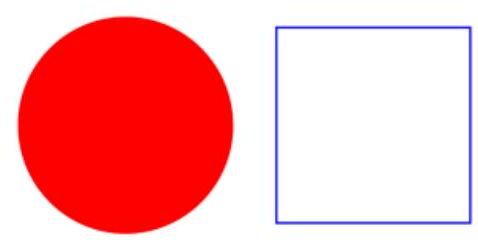
\includegraphics[width=\linewidth]{images/images/2024_12_29_858f09cde51177c71657g-27}
  
  JavaScript:
  
  \begin{verbatim}
  1 let circle = document.querySelector("circle")
  2 circle.setAttribute("fill","cyan")
  \end{verbatim}
  
  \section*{Canvas}
  \begin{itemize}
    \item Element canvas als Zeichenbereich im Dokument
    \item API zum Zeichnen auf dem Canvas
  \end{itemize}
  
  \begin{verbatim}
  <canvas></canvas>
  <script>
      Let cx = document.querySelector("canvas").getContext("2d")
      cx.beginPath()
      cx.moveTo(50, 10)
      cx.lineTo(10, 70)
      cx.lineTo(90, 70)
      cx.fill()
      let img = document.createElement("img")
      img.src = "img/hat.png"
      img.addEventListener("load" , () => {
          for (let x = 10; x < 200; x += 30) {
              cx.drawImage(img, x, 10)
          }
      })
  </script>
  \end{verbatim}
  
  Canvas Methoden
  
  \begin{center}
  \begin{tabular}{|l|l|}
  \hline
  Methoden & Beschreibung \\
  \hline
  scale & Skalieren \\
  \hline
  translate & Koordinatensystem verschieben \\
  \hline
  rotate & Koordinatensystem rotieren \\
  \hline
  save & Transformationen auf Stack speichern \\
  \hline
  restore & Letzten Zustand wiederherstellen \\
  \hline
  \end{tabular}
  \end{center}
  
  Browser-API\\
  Web Storage\\
  Web Storage speichert Daten auf der Seite des Client.
  
  \section*{Local Storage}
  Local Storage wird verwendet, um Daten der Webseite lokal abzuspeichern. Die Daten bleiben nach dem Schliessen des Browsers erhalten. Die Daten sind in Developer Tools einsehbar und änderbar.
  
  Die Daten werden nach Domains abgespeichert. Es können pro Webseite etwa 5MB abgespeichert werden.
  
  \begin{verbatim}
  1 localStorage.setItem("username","bkrt")
  2 console.log(localStorage.getItem("username")) // -> bkrt
  3 localStorage.removeItem("username")
  \end{verbatim}
  
  Die Werte werden als Strings gespeichert, daher müssen Objekte mit JSON codiert werden:\\
  1 Let user = \{name: "Hans", highscore: 234\}\\
  2 localStorage.setItem(JSON.stringify(user))
  
  \section*{History}
  History gibt zugriff auf den Verlauf des akutellen Fensters/Tab.
  
  \begin{verbatim}
  1 function goBack() {
  2 window.history.back();
  3
      ,}
  \end{verbatim}
  
  \begin{center}
  \begin{tabular}{|l|l|}
  \hline
  Methoden & Beschreibung \\
  \hline
  length (Attribut) & \begin{tabular}{l}
  Anzahl Einträgte inkl. aktueller Seite. Keine \\
  Methode! \\
  \end{tabular} \\
  \hline
  back & zurück zur letzten Seite \\
  \hline
  \end{tabular}
  \end{center}
  
  GeoLocation\\
  Mit der GeoLocation-API kann der Standort abgefragt werden.
  
  \begin{verbatim}
  var options = { enableHighAccuracy: true, timeout: 5000, maximumAge: 0 }
  function success(pos) {
      var crd = pos.coords
      console.log(`Latitude : ${crd.latitude}`)
      console.log(`Longitude: ${crd.longitude}`)
      console.log(`More or less ${crd.accuracy} meters.`)
  }
  function error(err) { ... }
  navigator.geolocation.getCurrentPosition(success, error, options)
  \end{verbatim}

\subsubsection{Client-Server-Interaktion}

\section*{Formulare}
Formulare ermöglichen Benutzereingaben. Sie gilt als Grundlade für Interaktion mit dem Web.\\
Input types:

\begin{itemize}
  \item submit, number, text, password, email, url , range , date , search , color
\end{itemize}

\begin{verbatim}
<form>
    <fieldset>
        <legend>General information</legend>
        <label>Text field <input type="text" value="hi"></label>
        <label>Password <input type="password" value="hi"></label>
        <label class="area">Textarea <textarea>hi</textarea></label>
    </fieldset>
    <fieldset>
        <legend>Additional information</legend>
        <label>Checkbox <input type="checkbox"></label>
        <label>Radio button <input type="radio" name="demo" checked></label>
        <label>Another one <input type="radio" name="demo"></label>
    </fieldset>
    <form>
    <label>Button <button>Click me</button></label>
    <label>Select menu
    <select name="cars">
    <option value="volvo">Volvo</option>
    <option value="saab">Saab</option>
    <option value="fiat">Fiat</option>
    <option value="audi">Audi</option>
    </select>
    </label>
    <input type="submit" value="Send">
</form>
|'
\end{verbatim}

\begin{center}
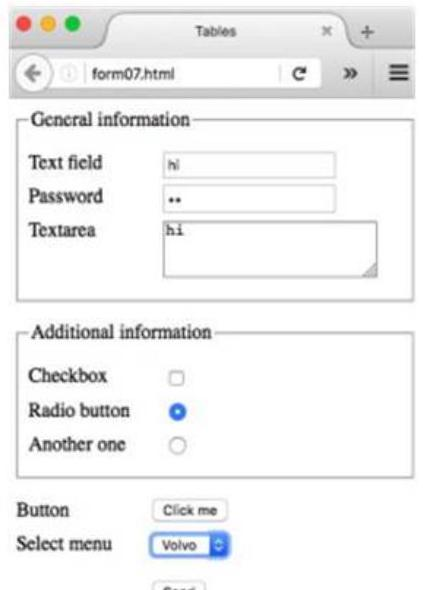
\includegraphics[width=\linewidth]{images/images/2024_12_29_858f09cde51177c71657g-29}
\end{center}

Formulare können auch POST/GET Aktionen ausführen:\\
Action beschreibt das Skript, welches die Daten annimmt. Method ist die Methode die ausgeführt wird.

\begin{verbatim}
<form action="/login" method="post">
2 ...
3 </form>
\end{verbatim}

\begin{center}
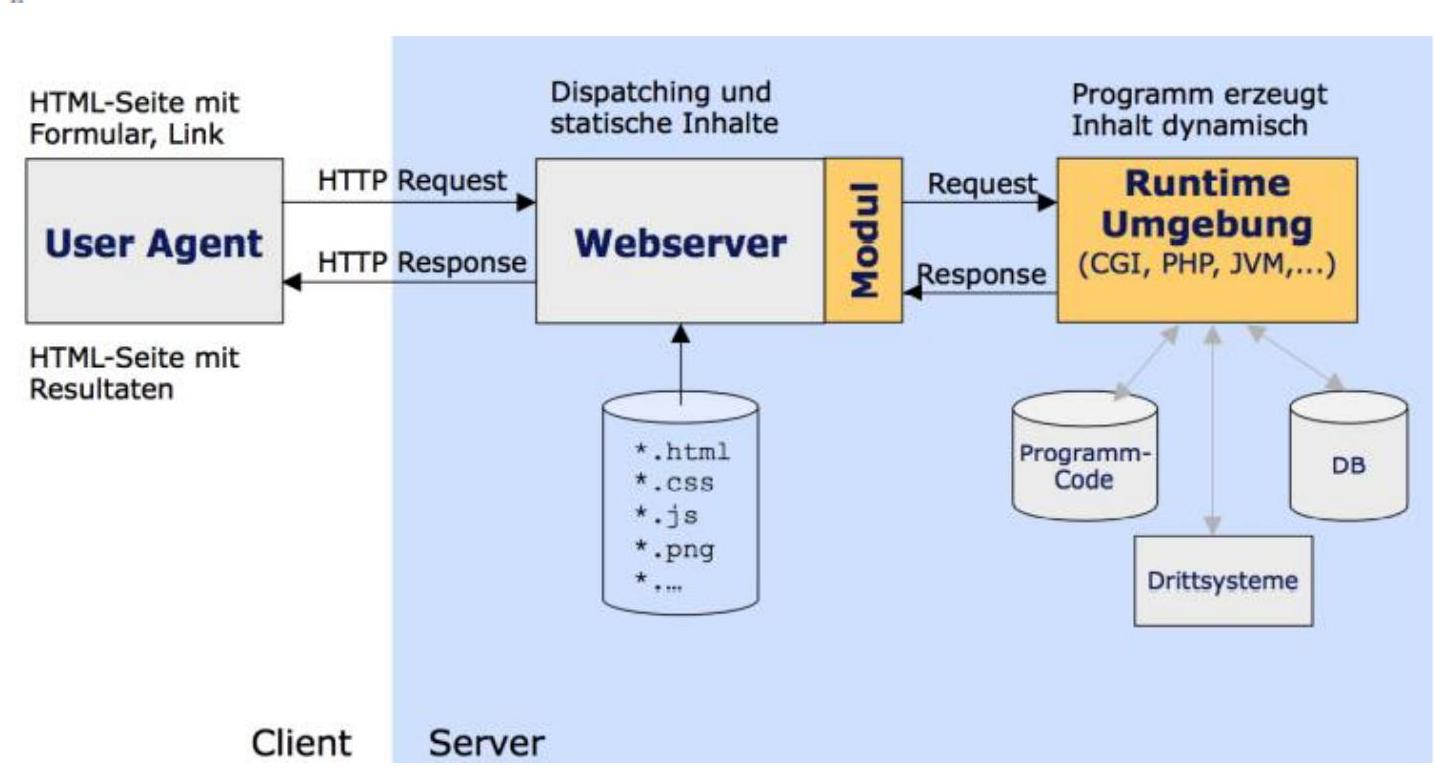
\includegraphics[width=\linewidth]{images/images/2024_12_29_858f09cde51177c71657g-29(1)}
\end{center}

Formular Events\\
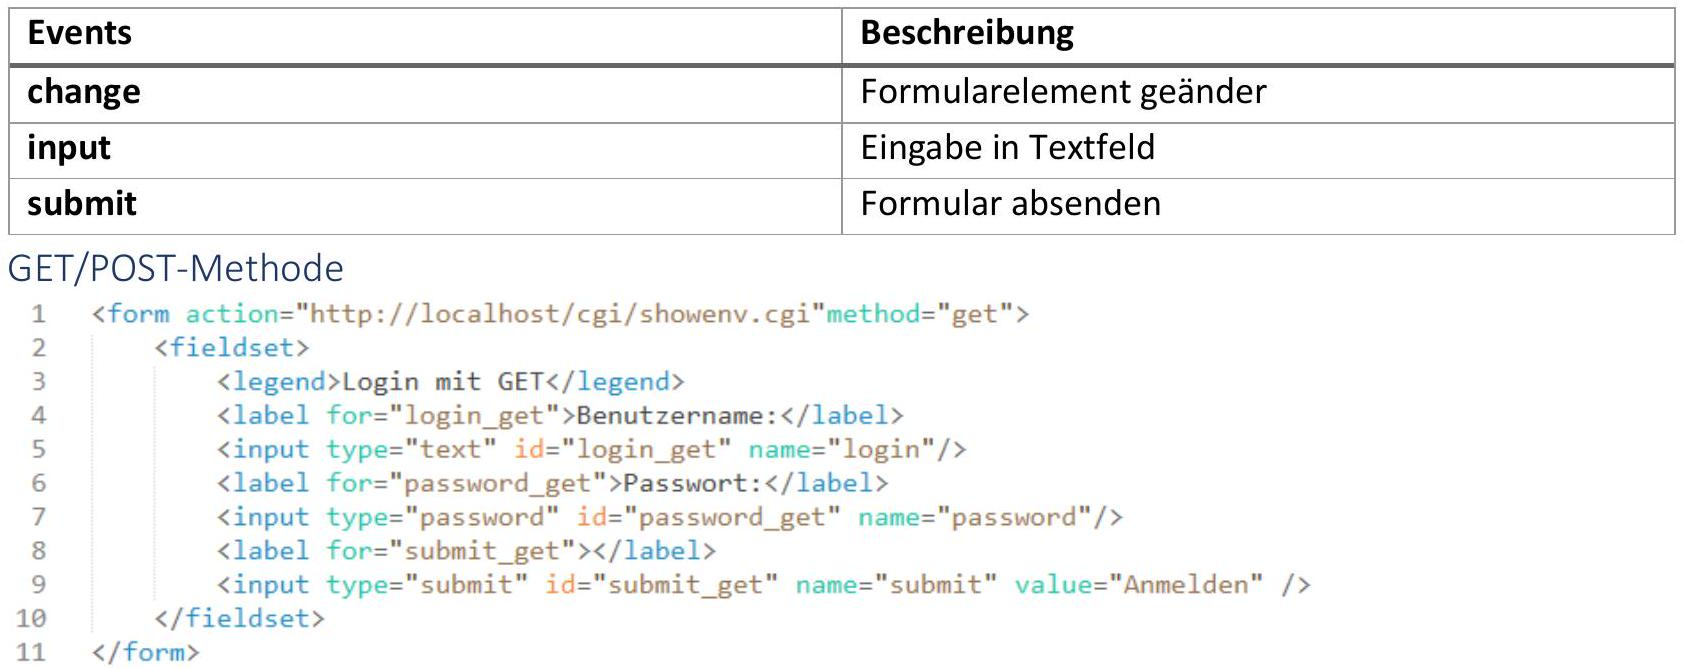
\includegraphics[width=\linewidth]{images/images/2024_12_29_858f09cde51177c71657g-30}

\section*{Cookies und Sessions}
Cookies

\begin{itemize}
  \item HTTP als zustandsloses Protokoll konzipiert
  \item Cookies: Speichern von Informationen auf dem Client
  \item Response: Set-Cookie -Header, Request: Cookie -Header
  \item Zugriff mit JavaScript möglich (ausser HttpOnly ist gesetzt)\\
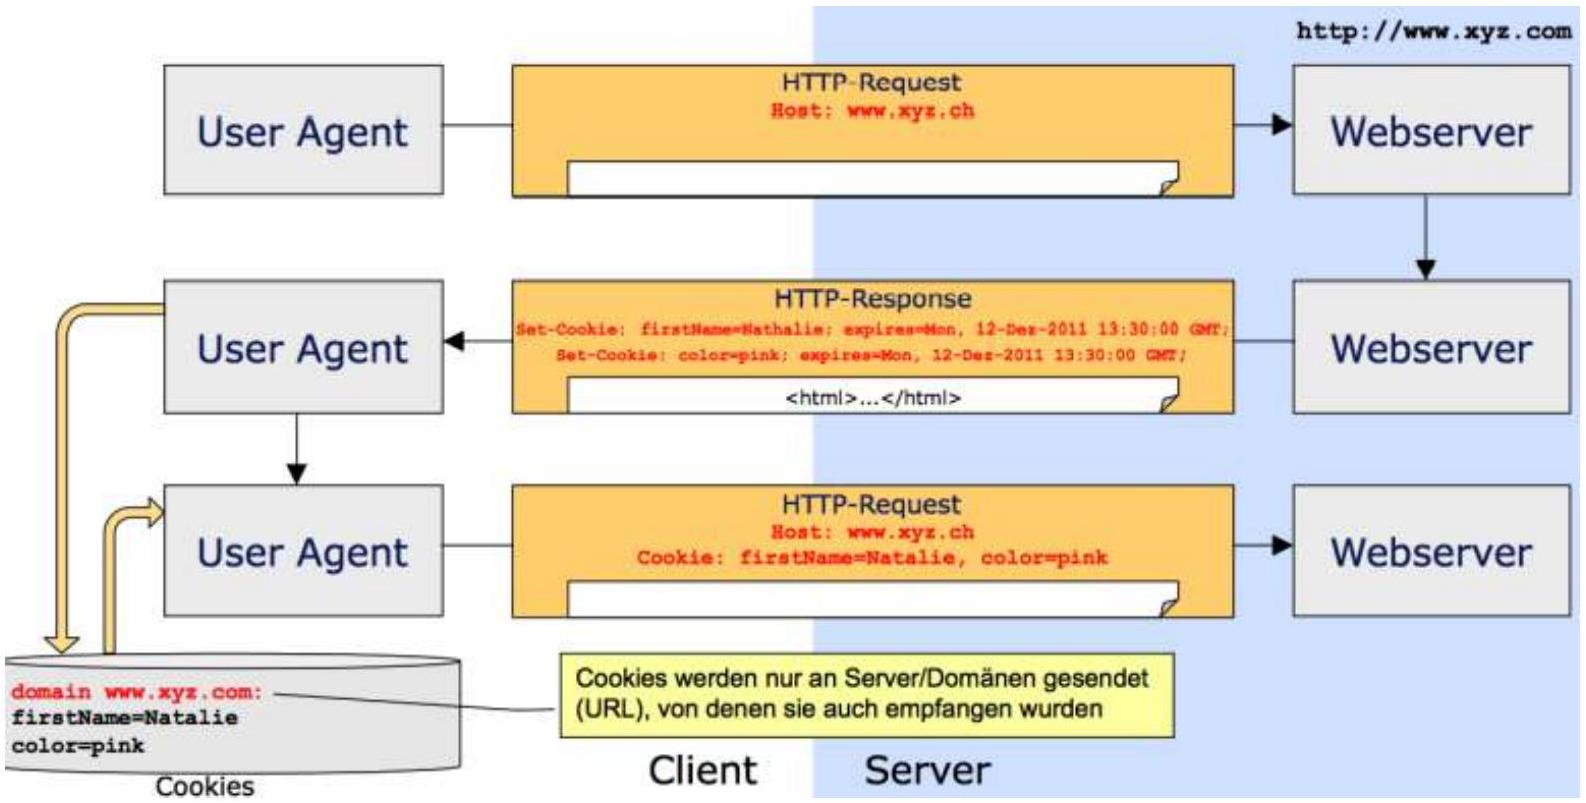
\includegraphics[width=\linewidth]{images/images/2024_12_29_858f09cde51177c71657g-31}
\end{itemize}

\section*{Sessions}
\begin{itemize}
  \item Cookies auf dem Client leicht manipulierbar
  \item Session: Client-spezifische Daten auf dem Server speichern
  \item Identifikation des Clients über Session-ID (Cookie o.a.)
  \item Gefahr: Session-ID gerät in falsche Hände (Session-Hijacking)
\end{itemize}

Ablauf:\\
\href{http://www.xyz.com}{http://www.xyz.com}\\
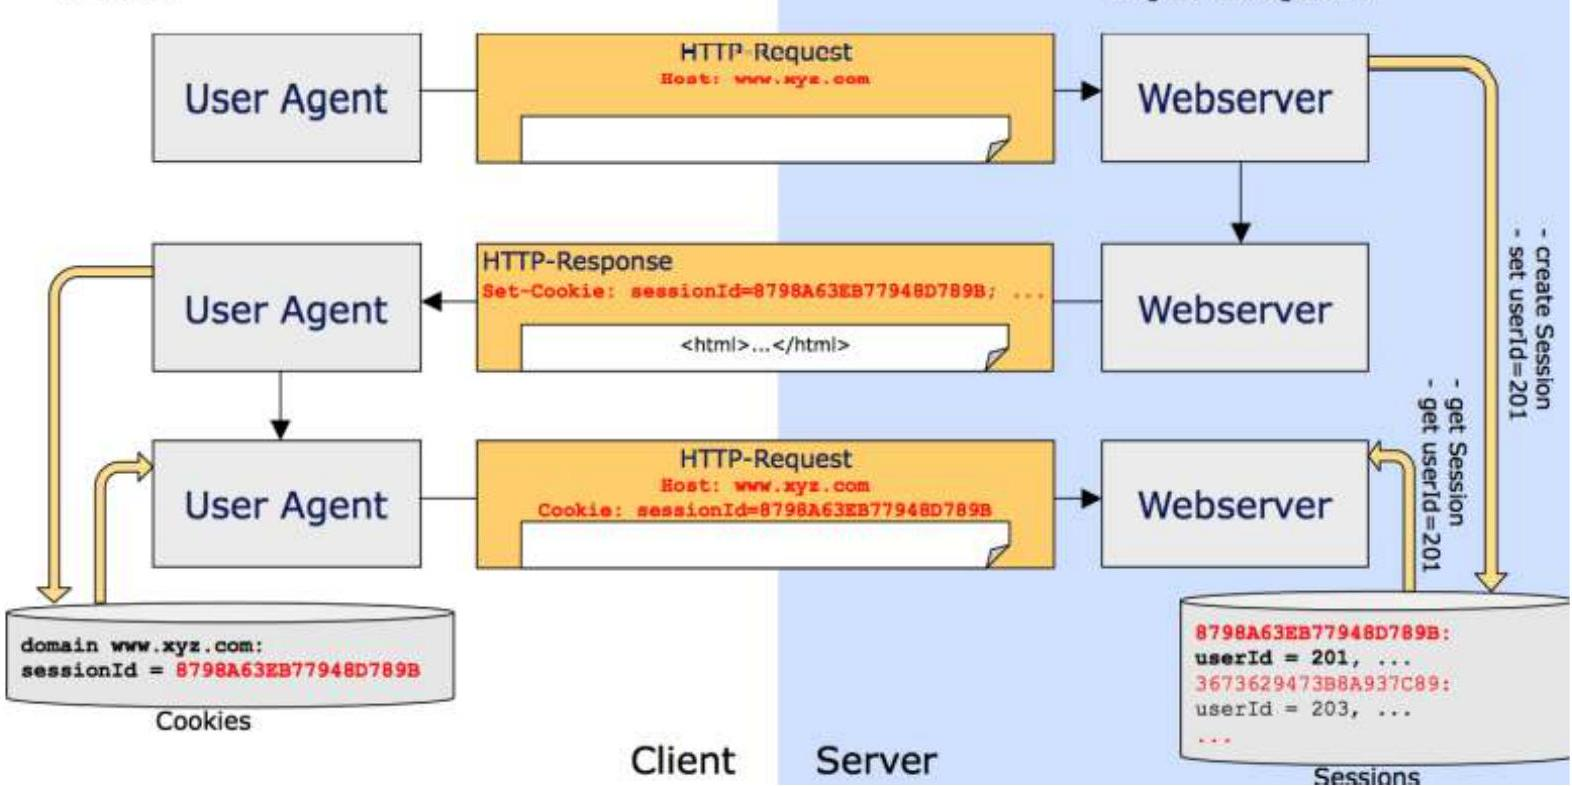
\includegraphics[width=\linewidth]{images/images/2024_12_29_858f09cde51177c71657g-31(1)}

\section*{Fetch API}
\begin{itemize}
  \item HTTP-Requests von JavaScripts
  \item Geben Promise zurück
  \item Nach Server-Antwort erfüllt mit Response-Objekt
\end{itemize}

\begin{verbatim}
fetch("example/data.txt")
.then(response => {
            console.log(response.status) // -> 200
    console.log(response.headers.get("Content-Type")) // -> text/plain
})
.then(resp => resp.text())
.then(text => console.log(text))
// -> This is the content of data.txt
\end{verbatim}

Response Objekt

\begin{itemize}
  \item headers : Zugriff auf HTTP-Header-Daten Methoden get, keys, forEach , ...
  \item status: Status-Code
  \item json() : liefert Promise mit Resultat der JSON-Verarbeitung
  \item text() : liefert Promise mit Inhalt der Server-Antwort
\end{itemize}